\section{Overview}

    \begin{figure}[H]
        \centering
        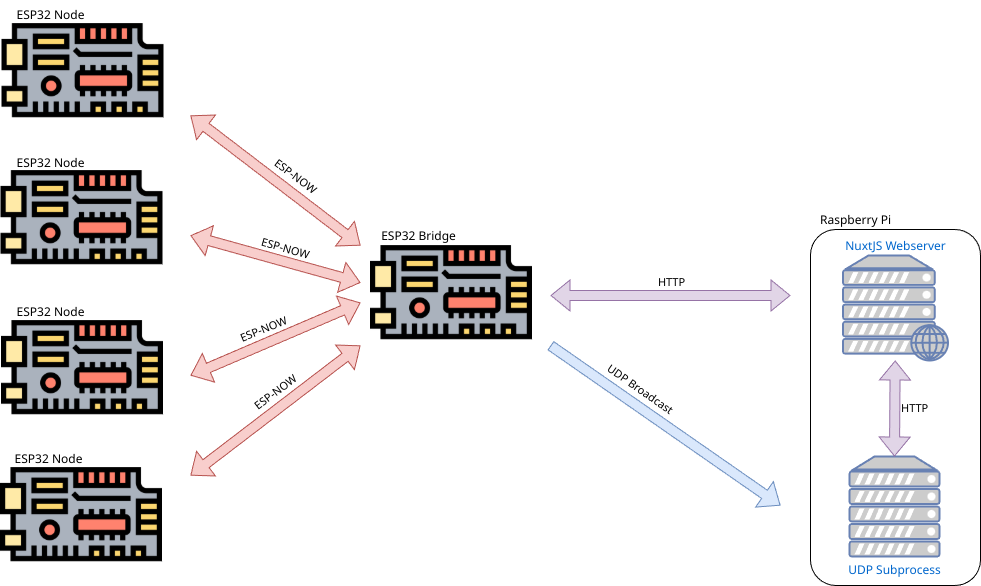
\includegraphics[width=0.9\textwidth]{topics/flowcharts/Networking.png}
        \caption{Networking Structure}
    \end{figure}
    \subsection{Web Server}
    A Nuxt.js Web server will function as the main interface
    for the user. It will communicate with the database and the
    dedicated Bridge-Node via HTTP. It should be capable of displaying
    and changing the state of the devices in the smart home.
    \subsection{Database}
    The database will store device states and measurements.
    Is can be read and written to by both the Web server and the
    Bridge-Node. 
    \subsection{Bridge-Node}
    The Bridge-Node will act as a bridge between everything running
    on the Raspberry Pi (Web server, database) and the ESP-NOW devices.
    It will be capable of receiving and sending data via both HTTP and
    ESP-NOW. It will also be responsible for discovering new ESP-NOW
    devices.